\documentclass[a4paper]{book}
\usepackage{makeidx}
\usepackage{graphicx}
\usepackage{multicol}
\usepackage{float}
\usepackage{listings}
\usepackage{color}
\usepackage{ifthen}
\usepackage[table]{xcolor}
\usepackage{textcomp}
\usepackage{alltt}
\usepackage{ifpdf}
\ifpdf
\usepackage[pdftex,
            pagebackref=true,
            colorlinks=true,
            linkcolor=blue,
            unicode
           ]{hyperref}
\else
\usepackage[ps2pdf,
            pagebackref=true,
            colorlinks=true,
            linkcolor=blue,
            unicode
           ]{hyperref}
\usepackage{pspicture}
\fi
\usepackage[utf8]{inputenc}
\usepackage{mathptmx}
\usepackage[scaled=.90]{helvet}
\usepackage{courier}
\usepackage{doxygen}
\lstset{language=C++,inputencoding=utf8,basicstyle=\footnotesize,breaklines=true,breakatwhitespace=true,tabsize=4,numbers=left }
\makeindex
\setcounter{tocdepth}{3}
\renewcommand{\footrulewidth}{0.4pt}
\begin{document}
\hypersetup{pageanchor=false}
\begin{titlepage}
\vspace*{7cm}
\begin{center}
{\Large GOGrapher \\[1ex]\large 2.0 }\\
\vspace*{1cm}
{\large Generated by Doxygen 1.7.3}\\
\vspace*{0.5cm}
{\small Fri Mar 18 2011 02:22:11}\\
\end{center}
\end{titlepage}
\clearemptydoublepage
\pagenumbering{roman}
\tableofcontents
\clearemptydoublepage
\pagenumbering{arabic}
\hypersetup{pageanchor=true}
\chapter{Namespace Index}
\section{Packages}
Here are the packages with brief descriptions (if available):\begin{DoxyCompactList}
\item\contentsline{section}{\hyperlink{namespace_g_o_gene_graph}{GOGeneGraph} }{\pageref{namespace_g_o_gene_graph}}{}
\item\contentsline{section}{\hyperlink{namespace_g_o_gene_pubmed_graph}{GOGenePubmedGraph} }{\pageref{namespace_g_o_gene_pubmed_graph}}{}
\item\contentsline{section}{\hyperlink{namespace_g_o_graph}{GOGraph} }{\pageref{namespace_g_o_graph}}{}
\item\contentsline{section}{\hyperlink{namespace_g_o_node}{GONode} }{\pageref{namespace_g_o_node}}{}
\item\contentsline{section}{\hyperlink{namespace_g_o_obo_xml_handler}{GOOboXmlHandler} }{\pageref{namespace_g_o_obo_xml_handler}}{}
\item\contentsline{section}{\hyperlink{namespace_g_o_pubmed_graph}{GOPubmedGraph} }{\pageref{namespace_g_o_pubmed_graph}}{}
\item\contentsline{section}{\hyperlink{namespacetest}{test} }{\pageref{namespacetest}}{}
\end{DoxyCompactList}

\chapter{Class Index}
\section{Class Hierarchy}
This inheritance list is sorted roughly, but not completely, alphabetically:\begin{DoxyCompactList}
\item \contentsline{section}{GOGraph.GOGraph}{\pageref{class_g_o_graph_1_1_g_o_graph}}{}
\begin{DoxyCompactList}
\item \contentsline{section}{GOGeneGraph.GOGeneGraph}{\pageref{class_g_o_gene_graph_1_1_g_o_gene_graph}}{}
\begin{DoxyCompactList}
\item \contentsline{section}{GOGenePubmedGraph.GOGenePubmedGraph}{\pageref{class_g_o_gene_pubmed_graph_1_1_g_o_gene_pubmed_graph}}{}
\end{DoxyCompactList}
\item \contentsline{section}{GOPubmedGraph.GOPubmedGraph}{\pageref{class_g_o_pubmed_graph_1_1_g_o_pubmed_graph}}{}
\begin{DoxyCompactList}
\item \contentsline{section}{GOGenePubmedGraph.GOGenePubmedGraph}{\pageref{class_g_o_gene_pubmed_graph_1_1_g_o_gene_pubmed_graph}}{}
\end{DoxyCompactList}
\end{DoxyCompactList}
\item \contentsline{section}{GONode.GONode}{\pageref{class_g_o_node_1_1_g_o_node}}{}
\item \contentsline{section}{GOOboXmlHandler.GOOboXmlHandler}{\pageref{class_g_o_obo_xml_handler_1_1_g_o_obo_xml_handler}}{}
\end{DoxyCompactList}

\chapter{Class Index}
\section{Class List}
Here are the classes, structs, unions and interfaces with brief descriptions:\begin{DoxyCompactList}
\item\contentsline{section}{\hyperlink{classgographer_1_1_corpus_1_1_corpus}{gographer.Corpus.Corpus} (A collection of \hyperlink{namespacegographer_1_1_document}{Document} objects )}{\pageref{classgographer_1_1_corpus_1_1_corpus}}{}
\item\contentsline{section}{\hyperlink{classgographer_1_1_document_1_1_document}{gographer.Document.Document} (A Python object representation of a PubMed record )}{\pageref{classgographer_1_1_document_1_1_document}}{}
\item\contentsline{section}{\hyperlink{classgographer_1_1_g_o_gene_graph_1_1_g_o_gene_graph}{gographer.GOGeneGraph.GOGeneGraph} }{\pageref{classgographer_1_1_g_o_gene_graph_1_1_g_o_gene_graph}}{}
\item\contentsline{section}{\hyperlink{classgographer_1_1_g_o_gene_pubmed_graph_1_1_g_o_gene_pubmed_graph}{gographer.GOGenePubmedGraph.GOGenePubmedGraph} }{\pageref{classgographer_1_1_g_o_gene_pubmed_graph_1_1_g_o_gene_pubmed_graph}}{}
\item\contentsline{section}{\hyperlink{classgographer_1_1_g_o_graph_1_1_g_o_graph}{gographer.GOGraph.GOGraph} }{\pageref{classgographer_1_1_g_o_graph_1_1_g_o_graph}}{}
\item\contentsline{section}{\hyperlink{classgographer_1_1_g_o_node_1_1_g_o_node}{gographer.GONode.GONode} }{\pageref{classgographer_1_1_g_o_node_1_1_g_o_node}}{}
\item\contentsline{section}{\hyperlink{classgographer_1_1_g_o_obo_xml_handler_1_1_g_o_obo_xml_handler}{gographer.GOOboXmlHandler.GOOboXmlHandler} }{\pageref{classgographer_1_1_g_o_obo_xml_handler_1_1_g_o_obo_xml_handler}}{}
\item\contentsline{section}{\hyperlink{classgographer_1_1_g_o_pubmed_graph_1_1_g_o_pubmed_graph}{gographer.GOPubmedGraph.GOPubmedGraph} }{\pageref{classgographer_1_1_g_o_pubmed_graph_1_1_g_o_pubmed_graph}}{}
\item\contentsline{section}{\hyperlink{classgographer_1_1_porter_stemmer_1_1_porter_stemmer}{gographer.PorterStemmer.PorterStemmer} }{\pageref{classgographer_1_1_porter_stemmer_1_1_porter_stemmer}}{}
\item\contentsline{section}{\hyperlink{classgographer_1_1_tokenizer_1_1_tokenizer}{gographer.Tokenizer.Tokenizer} }{\pageref{classgographer_1_1_tokenizer_1_1_tokenizer}}{}
\end{DoxyCompactList}

\chapter{File Index}
\section{File List}
Here is a list of all files with brief descriptions:\begin{DoxyCompactList}
\item\contentsline{section}{/Users/vickychen/Documents/Projects/myGOGrapher/gographer/\hyperlink{_g_o_gene_graph_8py}{GOGeneGraph.py} }{\pageref{_g_o_gene_graph_8py}}{}
\item\contentsline{section}{/Users/vickychen/Documents/Projects/myGOGrapher/gographer/\hyperlink{_g_o_gene_pubmed_graph_8py}{GOGenePubmedGraph.py} }{\pageref{_g_o_gene_pubmed_graph_8py}}{}
\item\contentsline{section}{/Users/vickychen/Documents/Projects/myGOGrapher/gographer/\hyperlink{_g_o_graph_8py}{GOGraph.py} }{\pageref{_g_o_graph_8py}}{}
\item\contentsline{section}{/Users/vickychen/Documents/Projects/myGOGrapher/gographer/\hyperlink{_g_o_node_8py}{GONode.py} }{\pageref{_g_o_node_8py}}{}
\item\contentsline{section}{/Users/vickychen/Documents/Projects/myGOGrapher/gographer/\hyperlink{_g_o_obo_xml_handler_8py}{GOOboXmlHandler.py} }{\pageref{_g_o_obo_xml_handler_8py}}{}
\item\contentsline{section}{/Users/vickychen/Documents/Projects/myGOGrapher/gographer/\hyperlink{_g_o_pubmed_graph_8py}{GOPubmedGraph.py} }{\pageref{_g_o_pubmed_graph_8py}}{}
\item\contentsline{section}{/Users/vickychen/Documents/Projects/myGOGrapher/gographer/\hyperlink{test_8py}{test.py} }{\pageref{test_8py}}{}
\end{DoxyCompactList}

\chapter{Namespace Documentation}
\hypertarget{namespace_g_o_gene_graph}{
\section{Package GOGeneGraph}
\label{namespace_g_o_gene_graph}\index{GOGeneGraph@{GOGeneGraph}}
}

\hypertarget{namespace_g_o_gene_pubmed_graph}{
\section{Package GOGenePubmedGraph}
\label{namespace_g_o_gene_pubmed_graph}\index{GOGenePubmedGraph@{GOGenePubmedGraph}}
}
\subsection*{Classes}
\begin{DoxyCompactItemize}
\item 
class \hyperlink{class_g_o_gene_pubmed_graph_1_1_g_o_gene_pubmed_graph}{GOGenePubmedGraph}
\end{DoxyCompactItemize}

\hypertarget{namespace_g_o_graph}{
\section{Package GOGraph}
\label{namespace_g_o_graph}\index{GOGraph@{GOGraph}}
}
\subsection*{Classes}
\begin{DoxyCompactItemize}
\item 
class \hyperlink{class_g_o_graph_1_1_g_o_graph}{GOGraph}
\end{DoxyCompactItemize}

\hypertarget{namespace_g_o_node}{
\section{Package GONode}
\label{namespace_g_o_node}\index{GONode@{GONode}}
}
\subsection*{Classes}
\begin{DoxyCompactItemize}
\item 
class \hyperlink{class_g_o_node_1_1_g_o_node}{GONode}
\end{DoxyCompactItemize}

\hypertarget{namespace_g_o_obo_xml_handler}{
\section{Package GOOboXmlHandler}
\label{namespace_g_o_obo_xml_handler}\index{GOOboXmlHandler@{GOOboXmlHandler}}
}
\subsection*{Classes}
\begin{DoxyCompactItemize}
\item 
class \hyperlink{class_g_o_obo_xml_handler_1_1_g_o_obo_xml_handler}{GOOboXmlHandler}
\end{DoxyCompactItemize}

\hypertarget{namespace_g_o_pubmed_graph}{
\section{Package GOPubmedGraph}
\label{namespace_g_o_pubmed_graph}\index{GOPubmedGraph@{GOPubmedGraph}}
}
\subsection*{Classes}
\begin{DoxyCompactItemize}
\item 
class \hyperlink{class_g_o_pubmed_graph_1_1_g_o_pubmed_graph}{GOPubmedGraph}
\end{DoxyCompactItemize}

\hypertarget{namespacetest}{
\section{Package test}
\label{namespacetest}\index{test@{test}}
}
\subsection*{Variables}
\begin{DoxyCompactItemize}
\item 
string \hyperlink{namespacetest_a0bae5ddd9b608f2179d9b18864638081}{location} = \char`\"{}./go\_\-daily-\/termdb.obo-\/xml\char`\"{}
\item 
tuple \hyperlink{namespacetest_a49256f3800de70e9aabf11ea0c3bb8e1}{GOGraphtest} = \hyperlink{class_g_o_graph_1_1_g_o_graph}{GOGraph}(\char`\"{}biological\_\-process\char`\"{}, location)
\end{DoxyCompactItemize}


\subsection{Variable Documentation}
\hypertarget{namespacetest_a49256f3800de70e9aabf11ea0c3bb8e1}{
\index{test@{test}!GOGraphtest@{GOGraphtest}}
\index{GOGraphtest@{GOGraphtest}!test@{test}}
\subsubsection[{GOGraphtest}]{\setlength{\rightskip}{0pt plus 5cm}tuple {\bf test.GOGraphtest} = {\bf GOGraph}(\char`\"{}biological\_\-process\char`\"{}, location)}}
\label{namespacetest_a49256f3800de70e9aabf11ea0c3bb8e1}
\hypertarget{namespacetest_a0bae5ddd9b608f2179d9b18864638081}{
\index{test@{test}!location@{location}}
\index{location@{location}!test@{test}}
\subsubsection[{location}]{\setlength{\rightskip}{0pt plus 5cm}string {\bf test.location} = \char`\"{}./go\_\-daily-\/termdb.obo-\/xml\char`\"{}}}
\label{namespacetest_a0bae5ddd9b608f2179d9b18864638081}

\chapter{Class Documentation}
\hypertarget{class_g_o_gene_graph_1_1_g_o_gene_graph}{
\section{GOGeneGraph.GOGeneGraph Class Reference}
\label{class_g_o_gene_graph_1_1_g_o_gene_graph}\index{GOGeneGraph::GOGeneGraph@{GOGeneGraph::GOGeneGraph}}
}
Inheritance diagram for GOGeneGraph.GOGeneGraph:\begin{figure}[H]
\begin{center}
\leavevmode
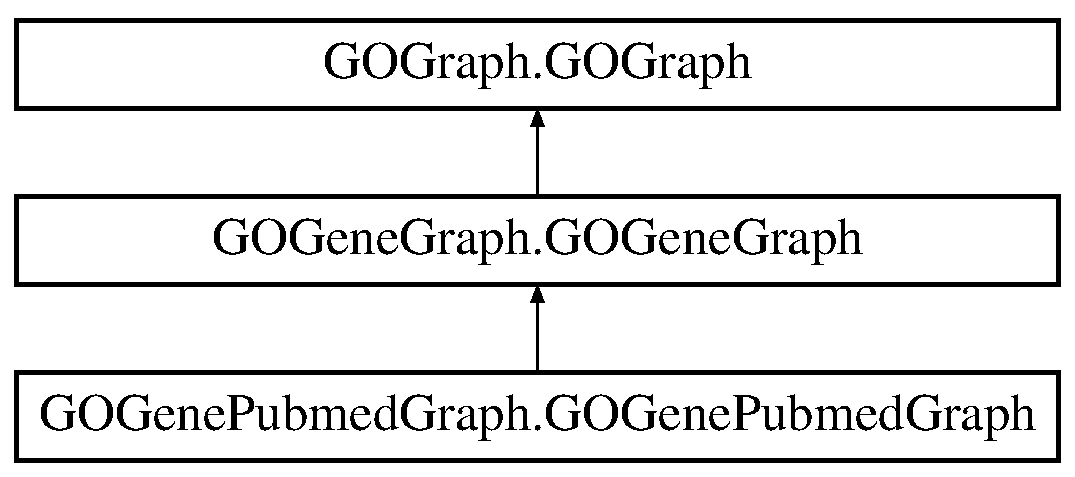
\includegraphics[height=3.000000cm]{class_g_o_gene_graph_1_1_g_o_gene_graph}
\end{center}
\end{figure}
\subsection*{Public Member Functions}
\begin{DoxyCompactItemize}
\item 
def \hyperlink{class_g_o_gene_graph_1_1_g_o_gene_graph_a37f579f2fd7c2e8f0e52345e5c94233f}{\_\-\_\-init\_\-\_\-}
\begin{DoxyCompactList}\small\item\em Create a gene graph from a \hyperlink{namespace_g_o_graph}{GOGraph}. \item\end{DoxyCompactList}\item 
def \hyperlink{class_g_o_gene_graph_1_1_g_o_gene_graph_a0881964964972853c93e7606b73bb825}{parseAssocFile}
\begin{DoxyCompactList}\small\item\em Parses the given association file and adds the gene information to the appropriate nodes. \item\end{DoxyCompactList}\item 
def \hyperlink{class_g_o_gene_graph_1_1_g_o_gene_graph_a276c7e223374b8c22417e195afacffed}{weight}
\begin{DoxyCompactList}\small\item\em Applies a weight to the graph. \item\end{DoxyCompactList}\item 
def \hyperlink{class_g_o_gene_graph_1_1_g_o_gene_graph_a5f437c2ab06eacde21831786192c4a4e}{toGOGenePubmedGraph}
\begin{DoxyCompactList}\small\item\em Returns a \hyperlink{namespace_g_o_gene_pubmed_graph}{GOGenePubmedGraph} version of itself. \item\end{DoxyCompactList}\item 
def \hyperlink{class_g_o_gene_graph_1_1_g_o_gene_graph_a778128e77640d18bcaf775c2348013d4}{getGenesByNode}
\begin{DoxyCompactList}\small\item\em Returns the associated genes for a given node. \item\end{DoxyCompactList}\item 
def \hyperlink{class_g_o_gene_graph_1_1_g_o_gene_graph_a6179a967c11a89a19dedb768cbb92bc9}{getPropagatedGenesByNode}
\begin{DoxyCompactList}\small\item\em Returns the associated propagated genes for a given node. \item\end{DoxyCompactList}\item 
def \hyperlink{class_g_o_gene_graph_1_1_g_o_gene_graph_a353497bb1605cfbefba350861e81ea6e}{getNodesByGene}
\begin{DoxyCompactList}\small\item\em Returns the associated nodes for a given gene. \item\end{DoxyCompactList}\item 
def \hyperlink{class_g_o_gene_graph_1_1_g_o_gene_graph_a3d0bfc52d583f576655cd0478ea2af86}{propagateGenes}
\begin{DoxyCompactList}\small\item\em Propagate the genes associated with each node to its parents. \item\end{DoxyCompactList}\end{DoxyCompactItemize}
\subsection*{Public Attributes}
\begin{DoxyCompactItemize}
\item 
\hyperlink{class_g_o_gene_graph_1_1_g_o_gene_graph_a6577e8fed9b4ff2629043ea62b73defe}{geneToNode}
\end{DoxyCompactItemize}


\subsection{Constructor \& Destructor Documentation}
\hypertarget{class_g_o_gene_graph_1_1_g_o_gene_graph_a37f579f2fd7c2e8f0e52345e5c94233f}{
\index{GOGeneGraph::GOGeneGraph@{GOGeneGraph::GOGeneGraph}!\_\-\_\-init\_\-\_\-@{\_\-\_\-init\_\-\_\-}}
\index{\_\-\_\-init\_\-\_\-@{\_\-\_\-init\_\-\_\-}!GOGeneGraph::GOGeneGraph@{GOGeneGraph::GOGeneGraph}}
\subsubsection[{\_\-\_\-init\_\-\_\-}]{\setlength{\rightskip}{0pt plus 5cm}def GOGeneGraph.GOGeneGraph.\_\-\_\-init\_\-\_\- (
\begin{DoxyParamCaption}
\item[{}]{self, }
\item[{}]{gograph, }
\item[{}]{assoc = {\ttfamily None}}
\end{DoxyParamCaption}
)}}
\label{class_g_o_gene_graph_1_1_g_o_gene_graph_a37f579f2fd7c2e8f0e52345e5c94233f}


Create a gene graph from a \hyperlink{namespace_g_o_graph}{GOGraph}. 


\begin{DoxyParams}{Parameters}
{\em gograph} & A \hyperlink{namespace_g_o_graph}{GOGraph} to base this graph off of \\
\hline
{\em assoc} & The file containing gene association information \\
\hline
\end{DoxyParams}


Reimplemented from \hyperlink{class_g_o_graph_1_1_g_o_graph_afc10d41165dd1ae6c4cce09102542122}{GOGraph.GOGraph}.



Reimplemented in \hyperlink{class_g_o_gene_pubmed_graph_1_1_g_o_gene_pubmed_graph_a903ad3047a2d1b88fffbdeee60b2045e}{GOGenePubmedGraph.GOGenePubmedGraph}.



\subsection{Member Function Documentation}
\hypertarget{class_g_o_gene_graph_1_1_g_o_gene_graph_a778128e77640d18bcaf775c2348013d4}{
\index{GOGeneGraph::GOGeneGraph@{GOGeneGraph::GOGeneGraph}!getGenesByNode@{getGenesByNode}}
\index{getGenesByNode@{getGenesByNode}!GOGeneGraph::GOGeneGraph@{GOGeneGraph::GOGeneGraph}}
\subsubsection[{getGenesByNode}]{\setlength{\rightskip}{0pt plus 5cm}def GOGeneGraph.GOGeneGraph.getGenesByNode (
\begin{DoxyParamCaption}
\item[{}]{self, }
\item[{}]{goid}
\end{DoxyParamCaption}
)}}
\label{class_g_o_gene_graph_1_1_g_o_gene_graph_a778128e77640d18bcaf775c2348013d4}


Returns the associated genes for a given node. 


\begin{DoxyParams}{Parameters}
{\em goid} & The GOID of the node to retrieve the associated genes from \\
\hline
\end{DoxyParams}
\hypertarget{class_g_o_gene_graph_1_1_g_o_gene_graph_a353497bb1605cfbefba350861e81ea6e}{
\index{GOGeneGraph::GOGeneGraph@{GOGeneGraph::GOGeneGraph}!getNodesByGene@{getNodesByGene}}
\index{getNodesByGene@{getNodesByGene}!GOGeneGraph::GOGeneGraph@{GOGeneGraph::GOGeneGraph}}
\subsubsection[{getNodesByGene}]{\setlength{\rightskip}{0pt plus 5cm}def GOGeneGraph.GOGeneGraph.getNodesByGene (
\begin{DoxyParamCaption}
\item[{}]{self, }
\item[{}]{geneid}
\end{DoxyParamCaption}
)}}
\label{class_g_o_gene_graph_1_1_g_o_gene_graph_a353497bb1605cfbefba350861e81ea6e}


Returns the associated nodes for a given gene. 


\begin{DoxyParams}{Parameters}
{\em geneid} & The ID of the gene for which to retrieve the associated nodes \\
\hline
\end{DoxyParams}
\hypertarget{class_g_o_gene_graph_1_1_g_o_gene_graph_a6179a967c11a89a19dedb768cbb92bc9}{
\index{GOGeneGraph::GOGeneGraph@{GOGeneGraph::GOGeneGraph}!getPropagatedGenesByNode@{getPropagatedGenesByNode}}
\index{getPropagatedGenesByNode@{getPropagatedGenesByNode}!GOGeneGraph::GOGeneGraph@{GOGeneGraph::GOGeneGraph}}
\subsubsection[{getPropagatedGenesByNode}]{\setlength{\rightskip}{0pt plus 5cm}def GOGeneGraph.GOGeneGraph.getPropagatedGenesByNode (
\begin{DoxyParamCaption}
\item[{}]{self, }
\item[{}]{goid}
\end{DoxyParamCaption}
)}}
\label{class_g_o_gene_graph_1_1_g_o_gene_graph_a6179a967c11a89a19dedb768cbb92bc9}


Returns the associated propagated genes for a given node. 


\begin{DoxyParams}{Parameters}
{\em goid} & The GOID of the node to retrieve the associated propagated genes from \\
\hline
\end{DoxyParams}
\hypertarget{class_g_o_gene_graph_1_1_g_o_gene_graph_a0881964964972853c93e7606b73bb825}{
\index{GOGeneGraph::GOGeneGraph@{GOGeneGraph::GOGeneGraph}!parseAssocFile@{parseAssocFile}}
\index{parseAssocFile@{parseAssocFile}!GOGeneGraph::GOGeneGraph@{GOGeneGraph::GOGeneGraph}}
\subsubsection[{parseAssocFile}]{\setlength{\rightskip}{0pt plus 5cm}def GOGeneGraph.GOGeneGraph.parseAssocFile (
\begin{DoxyParamCaption}
\item[{}]{self, }
\item[{}]{assoc}
\end{DoxyParamCaption}
)}}
\label{class_g_o_gene_graph_1_1_g_o_gene_graph_a0881964964972853c93e7606b73bb825}


Parses the given association file and adds the gene information to the appropriate nodes. 


\begin{DoxyParams}{Parameters}
{\em assoc} & The name of the association file to be parsed \\
\hline
\end{DoxyParams}
\hypertarget{class_g_o_gene_graph_1_1_g_o_gene_graph_a3d0bfc52d583f576655cd0478ea2af86}{
\index{GOGeneGraph::GOGeneGraph@{GOGeneGraph::GOGeneGraph}!propagateGenes@{propagateGenes}}
\index{propagateGenes@{propagateGenes}!GOGeneGraph::GOGeneGraph@{GOGeneGraph::GOGeneGraph}}
\subsubsection[{propagateGenes}]{\setlength{\rightskip}{0pt plus 5cm}def GOGeneGraph.GOGeneGraph.propagateGenes (
\begin{DoxyParamCaption}
\item[{}]{self}
\end{DoxyParamCaption}
)}}
\label{class_g_o_gene_graph_1_1_g_o_gene_graph_a3d0bfc52d583f576655cd0478ea2af86}


Propagate the genes associated with each node to its parents. 

\hypertarget{class_g_o_gene_graph_1_1_g_o_gene_graph_a5f437c2ab06eacde21831786192c4a4e}{
\index{GOGeneGraph::GOGeneGraph@{GOGeneGraph::GOGeneGraph}!toGOGenePubmedGraph@{toGOGenePubmedGraph}}
\index{toGOGenePubmedGraph@{toGOGenePubmedGraph}!GOGeneGraph::GOGeneGraph@{GOGeneGraph::GOGeneGraph}}
\subsubsection[{toGOGenePubmedGraph}]{\setlength{\rightskip}{0pt plus 5cm}def GOGeneGraph.GOGeneGraph.toGOGenePubmedGraph (
\begin{DoxyParamCaption}
\item[{}]{self}
\end{DoxyParamCaption}
)}}
\label{class_g_o_gene_graph_1_1_g_o_gene_graph_a5f437c2ab06eacde21831786192c4a4e}


Returns a \hyperlink{namespace_g_o_gene_pubmed_graph}{GOGenePubmedGraph} version of itself. 


\begin{DoxyParams}{Parameters}
{\em gopubmedgraph} & The \hyperlink{namespace_g_o_pubmed_graph}{GOPubmedGraph} that this graph is to be merged with \\
\hline
\end{DoxyParams}
\hypertarget{class_g_o_gene_graph_1_1_g_o_gene_graph_a276c7e223374b8c22417e195afacffed}{
\index{GOGeneGraph::GOGeneGraph@{GOGeneGraph::GOGeneGraph}!weight@{weight}}
\index{weight@{weight}!GOGeneGraph::GOGeneGraph@{GOGeneGraph::GOGeneGraph}}
\subsubsection[{weight}]{\setlength{\rightskip}{0pt plus 5cm}def GOGeneGraph.GOGeneGraph.weight (
\begin{DoxyParamCaption}
\item[{}]{self}
\end{DoxyParamCaption}
)}}
\label{class_g_o_gene_graph_1_1_g_o_gene_graph_a276c7e223374b8c22417e195afacffed}


Applies a weight to the graph. 



\subsection{Member Data Documentation}
\hypertarget{class_g_o_gene_graph_1_1_g_o_gene_graph_a6577e8fed9b4ff2629043ea62b73defe}{
\index{GOGeneGraph::GOGeneGraph@{GOGeneGraph::GOGeneGraph}!geneToNode@{geneToNode}}
\index{geneToNode@{geneToNode}!GOGeneGraph::GOGeneGraph@{GOGeneGraph::GOGeneGraph}}
\subsubsection[{geneToNode}]{\setlength{\rightskip}{0pt plus 5cm}{\bf GOGeneGraph.GOGeneGraph.geneToNode}}}
\label{class_g_o_gene_graph_1_1_g_o_gene_graph_a6577e8fed9b4ff2629043ea62b73defe}


The documentation for this class was generated from the following file:\begin{DoxyCompactItemize}
\item 
/Users/vickychen/Documents/Projects/myGOGrapher/gographer/\hyperlink{_g_o_gene_graph_8py}{GOGeneGraph.py}\end{DoxyCompactItemize}

\hypertarget{class_g_o_gene_pubmed_graph_1_1_g_o_gene_pubmed_graph}{
\section{GOGenePubmedGraph.GOGenePubmedGraph Class Reference}
\label{class_g_o_gene_pubmed_graph_1_1_g_o_gene_pubmed_graph}\index{GOGenePubmedGraph::GOGenePubmedGraph@{GOGenePubmedGraph::GOGenePubmedGraph}}
}
Inheritance diagram for GOGenePubmedGraph.GOGenePubmedGraph:\begin{figure}[H]
\begin{center}
\leavevmode
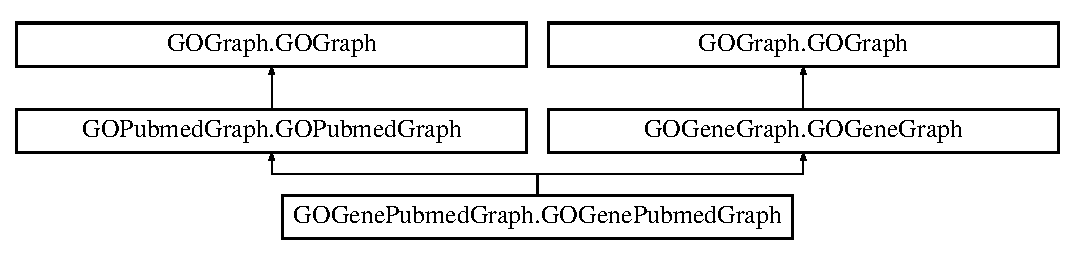
\includegraphics[height=2.978723cm]{class_g_o_gene_pubmed_graph_1_1_g_o_gene_pubmed_graph}
\end{center}
\end{figure}
\subsection*{Public Member Functions}
\begin{DoxyCompactItemize}
\item 
def \hyperlink{class_g_o_gene_pubmed_graph_1_1_g_o_gene_pubmed_graph_a903ad3047a2d1b88fffbdeee60b2045e}{\_\-\_\-init\_\-\_\-}
\begin{DoxyCompactList}\small\item\em Create a gene pubmed graph from a GOPubmedGraph and GOGeneGraph. \item\end{DoxyCompactList}\item 
def \hyperlink{class_g_o_gene_pubmed_graph_1_1_g_o_gene_pubmed_graph_a9eb2cec10a76d3b4e8022184c4260add}{weight}
\begin{DoxyCompactList}\small\item\em Weights the gene pubmed graph based off of the weight factor. \item\end{DoxyCompactList}\end{DoxyCompactItemize}


\subsection{Constructor \& Destructor Documentation}
\hypertarget{class_g_o_gene_pubmed_graph_1_1_g_o_gene_pubmed_graph_a903ad3047a2d1b88fffbdeee60b2045e}{
\index{GOGenePubmedGraph::GOGenePubmedGraph@{GOGenePubmedGraph::GOGenePubmedGraph}!\_\-\_\-init\_\-\_\-@{\_\-\_\-init\_\-\_\-}}
\index{\_\-\_\-init\_\-\_\-@{\_\-\_\-init\_\-\_\-}!GOGenePubmedGraph::GOGenePubmedGraph@{GOGenePubmedGraph::GOGenePubmedGraph}}
\subsubsection[{\_\-\_\-init\_\-\_\-}]{\setlength{\rightskip}{0pt plus 5cm}def GOGenePubmedGraph.GOGenePubmedGraph.\_\-\_\-init\_\-\_\- (
\begin{DoxyParamCaption}
\item[{}]{self, }
\item[{}]{gopubmedgraph, }
\item[{}]{gogenegraph}
\end{DoxyParamCaption}
)}}
\label{class_g_o_gene_pubmed_graph_1_1_g_o_gene_pubmed_graph_a903ad3047a2d1b88fffbdeee60b2045e}


Create a gene pubmed graph from a GOPubmedGraph and GOGeneGraph. 


\begin{DoxyParams}{Parameters}
{\em gopubmedgraph} & The GOPubmedGraph that should be merged to form the gene pubmed graph \\
\hline
{\em gogenegraph} & The GOGeneGraph that should be merged to form the gene pubmed graph \\
\hline
\end{DoxyParams}


Reimplemented from \hyperlink{class_g_o_gene_graph_1_1_g_o_gene_graph_a37f579f2fd7c2e8f0e52345e5c94233f}{GOGeneGraph.GOGeneGraph}.



\subsection{Member Function Documentation}
\hypertarget{class_g_o_gene_pubmed_graph_1_1_g_o_gene_pubmed_graph_a9eb2cec10a76d3b4e8022184c4260add}{
\index{GOGenePubmedGraph::GOGenePubmedGraph@{GOGenePubmedGraph::GOGenePubmedGraph}!weight@{weight}}
\index{weight@{weight}!GOGenePubmedGraph::GOGenePubmedGraph@{GOGenePubmedGraph::GOGenePubmedGraph}}
\subsubsection[{weight}]{\setlength{\rightskip}{0pt plus 5cm}def GOGenePubmedGraph.GOGenePubmedGraph.weight (
\begin{DoxyParamCaption}
\item[{}]{self, }
\item[{}]{weightFactor}
\end{DoxyParamCaption}
)}}
\label{class_g_o_gene_pubmed_graph_1_1_g_o_gene_pubmed_graph_a9eb2cec10a76d3b4e8022184c4260add}


Weights the gene pubmed graph based off of the weight factor. 


\begin{DoxyParams}{Parameters}
{\em weightFactor} & The factor by which the proteins and semantic distances should be weighted \\
\hline
\end{DoxyParams}


The documentation for this class was generated from the following file:\begin{DoxyCompactItemize}
\item 
Users/vickychen/Documents/Projects/myGOGrapher/gographer/GOGenePubmedGraph.py\end{DoxyCompactItemize}

\hypertarget{class_g_o_graph_1_1_g_o_graph}{
\section{GOGraph.GOGraph Class Reference}
\label{class_g_o_graph_1_1_g_o_graph}\index{GOGraph::GOGraph@{GOGraph::GOGraph}}
}
Inheritance diagram for GOGraph.GOGraph:\begin{figure}[H]
\begin{center}
\leavevmode
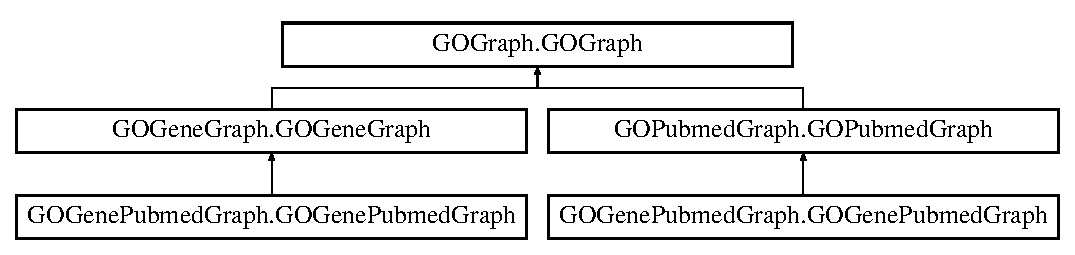
\includegraphics[height=2.978723cm]{class_g_o_graph_1_1_g_o_graph}
\end{center}
\end{figure}
\subsection*{Public Member Functions}
\begin{DoxyCompactItemize}
\item 
def \hyperlink{class_g_o_graph_1_1_g_o_graph_afc10d41165dd1ae6c4cce09102542122}{\_\-\_\-init\_\-\_\-}
\begin{DoxyCompactList}\small\item\em Constructor. \item\end{DoxyCompactList}\item 
def \hyperlink{class_g_o_graph_1_1_g_o_graph_ac368b1e74799f1947d195e3e2bf7074c}{parseOboXml}
\begin{DoxyCompactList}\small\item\em Parses the given OBO XML file and creates a \hyperlink{class_g_o_graph_1_1_g_o_graph}{GOGraph}. \item\end{DoxyCompactList}\item 
def \hyperlink{class_g_o_graph_1_1_g_o_graph_aff70b5975f6e755e3304cfc3d4ef91a0}{getLevel}
\begin{DoxyCompactList}\small\item\em Returns the minimum depth of the node. \item\end{DoxyCompactList}\item 
def \hyperlink{class_g_o_graph_1_1_g_o_graph_aeef340ff2a82454a8d92d9711fd7a92b}{getNameSpace}
\begin{DoxyCompactList}\small\item\em Returns the namespace of the graph. \item\end{DoxyCompactList}\item 
def \hyperlink{class_g_o_graph_1_1_g_o_graph_ad97c179c4ec3d79a3092810ba1fbc241}{savePickle}
\begin{DoxyCompactList}\small\item\em Save self using pickle protocol. \item\end{DoxyCompactList}\item 
def \hyperlink{class_g_o_graph_1_1_g_o_graph_ada6b7d590cfca9d4baec8d082577ac21}{loadPickle}
\begin{DoxyCompactList}\small\item\em Load a pickle from the filesystem. \item\end{DoxyCompactList}\item 
def \hyperlink{class_g_o_graph_1_1_g_o_graph_a09e8d05c3bbf4e7f6ae1bbbac535e2f2}{getNodeDescription}
\begin{DoxyCompactList}\small\item\em Get the description of a node. \item\end{DoxyCompactList}\item 
def \hyperlink{class_g_o_graph_1_1_g_o_graph_afea5ecb3c758e65a54f0167d11c1ad5a}{getNodeNamespace}
\begin{DoxyCompactList}\small\item\em Get the description of a node. \item\end{DoxyCompactList}\end{DoxyCompactItemize}
\subsection*{Public Attributes}
\begin{DoxyCompactItemize}
\item 
\hyperlink{class_g_o_graph_1_1_g_o_graph_af17f1eca2d2734e36976754e8ad4582a}{namespace}
\end{DoxyCompactItemize}


\subsection{Constructor \& Destructor Documentation}
\hypertarget{class_g_o_graph_1_1_g_o_graph_afc10d41165dd1ae6c4cce09102542122}{
\index{GOGraph::GOGraph@{GOGraph::GOGraph}!\_\-\_\-init\_\-\_\-@{\_\-\_\-init\_\-\_\-}}
\index{\_\-\_\-init\_\-\_\-@{\_\-\_\-init\_\-\_\-}!GOGraph::GOGraph@{GOGraph::GOGraph}}
\subsubsection[{\_\-\_\-init\_\-\_\-}]{\setlength{\rightskip}{0pt plus 5cm}def GOGraph.GOGraph.\_\-\_\-init\_\-\_\- (
\begin{DoxyParamCaption}
\item[{}]{self, }
\item[{}]{namespace = {\ttfamily None}, }
\item[{}]{GOOboXmlFileName = {\ttfamily None}}
\end{DoxyParamCaption}
)}}
\label{class_g_o_graph_1_1_g_o_graph_afc10d41165dd1ae6c4cce09102542122}


Constructor. 


\begin{DoxyParams}{Parameters}
{\em namespace} & The branch of the GO ontology stored by this graph \\
\hline
{\em XMLFileName} & The file contains the GO definition in the format of the OBO in XML \\
\hline
\end{DoxyParams}


Reimplemented in \hyperlink{class_g_o_gene_graph_1_1_g_o_gene_graph_a37f579f2fd7c2e8f0e52345e5c94233f}{GOGeneGraph.GOGeneGraph}, and \hyperlink{class_g_o_gene_pubmed_graph_1_1_g_o_gene_pubmed_graph_a903ad3047a2d1b88fffbdeee60b2045e}{GOGenePubmedGraph.GOGenePubmedGraph}.



\subsection{Member Function Documentation}
\hypertarget{class_g_o_graph_1_1_g_o_graph_aff70b5975f6e755e3304cfc3d4ef91a0}{
\index{GOGraph::GOGraph@{GOGraph::GOGraph}!getLevel@{getLevel}}
\index{getLevel@{getLevel}!GOGraph::GOGraph@{GOGraph::GOGraph}}
\subsubsection[{getLevel}]{\setlength{\rightskip}{0pt plus 5cm}def GOGraph.GOGraph.getLevel (
\begin{DoxyParamCaption}
\item[{}]{self, }
\item[{}]{goid}
\end{DoxyParamCaption}
)}}
\label{class_g_o_graph_1_1_g_o_graph_aff70b5975f6e755e3304cfc3d4ef91a0}


Returns the minimum depth of the node. 


\begin{DoxyParams}{Parameters}
{\em goid} & The GO ID of the node whose depth will be found and returned \\
\hline
\end{DoxyParams}
\hypertarget{class_g_o_graph_1_1_g_o_graph_aeef340ff2a82454a8d92d9711fd7a92b}{
\index{GOGraph::GOGraph@{GOGraph::GOGraph}!getNameSpace@{getNameSpace}}
\index{getNameSpace@{getNameSpace}!GOGraph::GOGraph@{GOGraph::GOGraph}}
\subsubsection[{getNameSpace}]{\setlength{\rightskip}{0pt plus 5cm}def GOGraph.GOGraph.getNameSpace (
\begin{DoxyParamCaption}
\item[{}]{self}
\end{DoxyParamCaption}
)}}
\label{class_g_o_graph_1_1_g_o_graph_aeef340ff2a82454a8d92d9711fd7a92b}


Returns the namespace of the graph. 

\hypertarget{class_g_o_graph_1_1_g_o_graph_a09e8d05c3bbf4e7f6ae1bbbac535e2f2}{
\index{GOGraph::GOGraph@{GOGraph::GOGraph}!getNodeDescription@{getNodeDescription}}
\index{getNodeDescription@{getNodeDescription}!GOGraph::GOGraph@{GOGraph::GOGraph}}
\subsubsection[{getNodeDescription}]{\setlength{\rightskip}{0pt plus 5cm}def GOGraph.GOGraph.getNodeDescription (
\begin{DoxyParamCaption}
\item[{}]{self, }
\item[{}]{goid}
\end{DoxyParamCaption}
)}}
\label{class_g_o_graph_1_1_g_o_graph_a09e8d05c3bbf4e7f6ae1bbbac535e2f2}


Get the description of a node. 


\begin{DoxyParams}{Parameters}
{\em goid} & The GO ID of the node to get the description of \\
\hline
\end{DoxyParams}
\hypertarget{class_g_o_graph_1_1_g_o_graph_afea5ecb3c758e65a54f0167d11c1ad5a}{
\index{GOGraph::GOGraph@{GOGraph::GOGraph}!getNodeNamespace@{getNodeNamespace}}
\index{getNodeNamespace@{getNodeNamespace}!GOGraph::GOGraph@{GOGraph::GOGraph}}
\subsubsection[{getNodeNamespace}]{\setlength{\rightskip}{0pt plus 5cm}def GOGraph.GOGraph.getNodeNamespace (
\begin{DoxyParamCaption}
\item[{}]{self, }
\item[{}]{goid}
\end{DoxyParamCaption}
)}}
\label{class_g_o_graph_1_1_g_o_graph_afea5ecb3c758e65a54f0167d11c1ad5a}


Get the description of a node. 


\begin{DoxyParams}{Parameters}
{\em goid} & The GO ID of the node to get the description of \\
\hline
\end{DoxyParams}
\hypertarget{class_g_o_graph_1_1_g_o_graph_ada6b7d590cfca9d4baec8d082577ac21}{
\index{GOGraph::GOGraph@{GOGraph::GOGraph}!loadPickle@{loadPickle}}
\index{loadPickle@{loadPickle}!GOGraph::GOGraph@{GOGraph::GOGraph}}
\subsubsection[{loadPickle}]{\setlength{\rightskip}{0pt plus 5cm}def GOGraph.GOGraph.loadPickle (
\begin{DoxyParamCaption}
\item[{}]{klass, }
\item[{}]{filename = {\ttfamily \char`\"{}gograph.pickle\char`\"{}}}
\end{DoxyParamCaption}
)}}
\label{class_g_o_graph_1_1_g_o_graph_ada6b7d590cfca9d4baec8d082577ac21}


Load a pickle from the filesystem. 


\begin{DoxyParams}{Parameters}
{\em filename} & The location of the pickle file to load \\
\hline
\end{DoxyParams}
\hypertarget{class_g_o_graph_1_1_g_o_graph_ac368b1e74799f1947d195e3e2bf7074c}{
\index{GOGraph::GOGraph@{GOGraph::GOGraph}!parseOboXml@{parseOboXml}}
\index{parseOboXml@{parseOboXml}!GOGraph::GOGraph@{GOGraph::GOGraph}}
\subsubsection[{parseOboXml}]{\setlength{\rightskip}{0pt plus 5cm}def GOGraph.GOGraph.parseOboXml (
\begin{DoxyParamCaption}
\item[{}]{self, }
\item[{}]{GOOboXmlFileName}
\end{DoxyParamCaption}
)}}
\label{class_g_o_graph_1_1_g_o_graph_ac368b1e74799f1947d195e3e2bf7074c}


Parses the given OBO XML file and creates a \hyperlink{class_g_o_graph_1_1_g_o_graph}{GOGraph}. 


\begin{DoxyParams}{Parameters}
{\em GOOboXMLFileName} & The name of the OBO XML file to be parsed \\
\hline
\end{DoxyParams}
\hypertarget{class_g_o_graph_1_1_g_o_graph_ad97c179c4ec3d79a3092810ba1fbc241}{
\index{GOGraph::GOGraph@{GOGraph::GOGraph}!savePickle@{savePickle}}
\index{savePickle@{savePickle}!GOGraph::GOGraph@{GOGraph::GOGraph}}
\subsubsection[{savePickle}]{\setlength{\rightskip}{0pt plus 5cm}def GOGraph.GOGraph.savePickle (
\begin{DoxyParamCaption}
\item[{}]{self, }
\item[{}]{filename = {\ttfamily \char`\"{}gograph.pickle\char`\"{}}}
\end{DoxyParamCaption}
)}}
\label{class_g_o_graph_1_1_g_o_graph_ad97c179c4ec3d79a3092810ba1fbc241}


Save self using pickle protocol. 


\begin{DoxyParams}{Parameters}
{\em filename} & The filename of the pickle to use \\
\hline
\end{DoxyParams}


\subsection{Member Data Documentation}
\hypertarget{class_g_o_graph_1_1_g_o_graph_af17f1eca2d2734e36976754e8ad4582a}{
\index{GOGraph::GOGraph@{GOGraph::GOGraph}!namespace@{namespace}}
\index{namespace@{namespace}!GOGraph::GOGraph@{GOGraph::GOGraph}}
\subsubsection[{namespace}]{\setlength{\rightskip}{0pt plus 5cm}{\bf GOGraph.GOGraph.namespace}}}
\label{class_g_o_graph_1_1_g_o_graph_af17f1eca2d2734e36976754e8ad4582a}


The documentation for this class was generated from the following file:\begin{DoxyCompactItemize}
\item 
/Users/vickychen/Documents/Projects/myGOGrapher/gographer/\hyperlink{_g_o_graph_8py}{GOGraph.py}\end{DoxyCompactItemize}

\hypertarget{class_g_o_node_1_1_g_o_node}{
\section{GONode.GONode Class Reference}
\label{class_g_o_node_1_1_g_o_node}\index{GONode::GONode@{GONode::GONode}}
}
\subsection*{Public Member Functions}
\begin{DoxyCompactItemize}
\item 
def \hyperlink{class_g_o_node_1_1_g_o_node_aed2500c2cbac29cc9793c37396b75928}{\_\-\_\-init\_\-\_\-}
\item 
def \hyperlink{class_g_o_node_1_1_g_o_node_a7bc51e25200c46ad8a7557992f90f7ca}{setGOID}
\item 
def \hyperlink{class_g_o_node_1_1_g_o_node_a0590505c8573df5ef3b6e8290e821de1}{setNamespace}
\item 
def \hyperlink{class_g_o_node_1_1_g_o_node_adf32cb452b5eff47a658d83ef9ce9381}{setParents}
\item 
def \hyperlink{class_g_o_node_1_1_g_o_node_a038f04eff9f5d8486280bc70887515fa}{setObsolete}
\item 
def \hyperlink{class_g_o_node_1_1_g_o_node_ab48dc024009773f22884b5a7c75d17cd}{setName}
\item 
def \hyperlink{class_g_o_node_1_1_g_o_node_a6da2fec8371255c0728c3bed095ab4f9}{setDescription}
\end{DoxyCompactItemize}
\subsection*{Public Attributes}
\begin{DoxyCompactItemize}
\item 
\hyperlink{class_g_o_node_1_1_g_o_node_a419738231e6061c8f35c7038600045b5}{goid}
\item 
\hyperlink{class_g_o_node_1_1_g_o_node_a14d769d661d7dad68b451d0ee40dc7c8}{namespace}
\item 
\hyperlink{class_g_o_node_1_1_g_o_node_a0e5b6b8b5e9b4a88ff0752017d90f544}{parents}
\item 
\hyperlink{class_g_o_node_1_1_g_o_node_a21c9f4840075c55ca91a59d4e7907f1f}{obsolete}
\item 
\hyperlink{class_g_o_node_1_1_g_o_node_a18b00948dd27ef1af426a1b8a522467d}{name}
\item 
\hyperlink{class_g_o_node_1_1_g_o_node_ad22366488d580d7aa91527f0b592d64d}{description}
\end{DoxyCompactItemize}


\subsection{Constructor \& Destructor Documentation}
\hypertarget{class_g_o_node_1_1_g_o_node_aed2500c2cbac29cc9793c37396b75928}{
\index{GONode::GONode@{GONode::GONode}!\_\-\_\-init\_\-\_\-@{\_\-\_\-init\_\-\_\-}}
\index{\_\-\_\-init\_\-\_\-@{\_\-\_\-init\_\-\_\-}!GONode::GONode@{GONode::GONode}}
\subsubsection[{\_\-\_\-init\_\-\_\-}]{\setlength{\rightskip}{0pt plus 5cm}def GONode.GONode.\_\-\_\-init\_\-\_\- (
\begin{DoxyParamCaption}
\item[{}]{self, }
\item[{}]{goid = {\ttfamily None}, }
\item[{}]{namespace = {\ttfamily None}, }
\item[{}]{parents = {\ttfamily None}, }
\item[{}]{obsolete = {\ttfamily False}, }
\item[{}]{name = {\ttfamily None}, }
\item[{}]{description = {\ttfamily None}}
\end{DoxyParamCaption}
)}}
\label{class_g_o_node_1_1_g_o_node_aed2500c2cbac29cc9793c37396b75928}


\subsection{Member Function Documentation}
\hypertarget{class_g_o_node_1_1_g_o_node_a6da2fec8371255c0728c3bed095ab4f9}{
\index{GONode::GONode@{GONode::GONode}!setDescription@{setDescription}}
\index{setDescription@{setDescription}!GONode::GONode@{GONode::GONode}}
\subsubsection[{setDescription}]{\setlength{\rightskip}{0pt plus 5cm}def GONode.GONode.setDescription (
\begin{DoxyParamCaption}
\item[{}]{self, }
\item[{}]{description}
\end{DoxyParamCaption}
)}}
\label{class_g_o_node_1_1_g_o_node_a6da2fec8371255c0728c3bed095ab4f9}
\hypertarget{class_g_o_node_1_1_g_o_node_a7bc51e25200c46ad8a7557992f90f7ca}{
\index{GONode::GONode@{GONode::GONode}!setGOID@{setGOID}}
\index{setGOID@{setGOID}!GONode::GONode@{GONode::GONode}}
\subsubsection[{setGOID}]{\setlength{\rightskip}{0pt plus 5cm}def GONode.GONode.setGOID (
\begin{DoxyParamCaption}
\item[{}]{self, }
\item[{}]{goid}
\end{DoxyParamCaption}
)}}
\label{class_g_o_node_1_1_g_o_node_a7bc51e25200c46ad8a7557992f90f7ca}
\hypertarget{class_g_o_node_1_1_g_o_node_ab48dc024009773f22884b5a7c75d17cd}{
\index{GONode::GONode@{GONode::GONode}!setName@{setName}}
\index{setName@{setName}!GONode::GONode@{GONode::GONode}}
\subsubsection[{setName}]{\setlength{\rightskip}{0pt plus 5cm}def GONode.GONode.setName (
\begin{DoxyParamCaption}
\item[{}]{self, }
\item[{}]{name}
\end{DoxyParamCaption}
)}}
\label{class_g_o_node_1_1_g_o_node_ab48dc024009773f22884b5a7c75d17cd}
\hypertarget{class_g_o_node_1_1_g_o_node_a0590505c8573df5ef3b6e8290e821de1}{
\index{GONode::GONode@{GONode::GONode}!setNamespace@{setNamespace}}
\index{setNamespace@{setNamespace}!GONode::GONode@{GONode::GONode}}
\subsubsection[{setNamespace}]{\setlength{\rightskip}{0pt plus 5cm}def GONode.GONode.setNamespace (
\begin{DoxyParamCaption}
\item[{}]{self, }
\item[{}]{namespace}
\end{DoxyParamCaption}
)}}
\label{class_g_o_node_1_1_g_o_node_a0590505c8573df5ef3b6e8290e821de1}
\hypertarget{class_g_o_node_1_1_g_o_node_a038f04eff9f5d8486280bc70887515fa}{
\index{GONode::GONode@{GONode::GONode}!setObsolete@{setObsolete}}
\index{setObsolete@{setObsolete}!GONode::GONode@{GONode::GONode}}
\subsubsection[{setObsolete}]{\setlength{\rightskip}{0pt plus 5cm}def GONode.GONode.setObsolete (
\begin{DoxyParamCaption}
\item[{}]{self, }
\item[{}]{obsolete}
\end{DoxyParamCaption}
)}}
\label{class_g_o_node_1_1_g_o_node_a038f04eff9f5d8486280bc70887515fa}
\hypertarget{class_g_o_node_1_1_g_o_node_adf32cb452b5eff47a658d83ef9ce9381}{
\index{GONode::GONode@{GONode::GONode}!setParents@{setParents}}
\index{setParents@{setParents}!GONode::GONode@{GONode::GONode}}
\subsubsection[{setParents}]{\setlength{\rightskip}{0pt plus 5cm}def GONode.GONode.setParents (
\begin{DoxyParamCaption}
\item[{}]{self, }
\item[{}]{parents}
\end{DoxyParamCaption}
)}}
\label{class_g_o_node_1_1_g_o_node_adf32cb452b5eff47a658d83ef9ce9381}


\subsection{Member Data Documentation}
\hypertarget{class_g_o_node_1_1_g_o_node_ad22366488d580d7aa91527f0b592d64d}{
\index{GONode::GONode@{GONode::GONode}!description@{description}}
\index{description@{description}!GONode::GONode@{GONode::GONode}}
\subsubsection[{description}]{\setlength{\rightskip}{0pt plus 5cm}{\bf GONode.GONode.description}}}
\label{class_g_o_node_1_1_g_o_node_ad22366488d580d7aa91527f0b592d64d}
\hypertarget{class_g_o_node_1_1_g_o_node_a419738231e6061c8f35c7038600045b5}{
\index{GONode::GONode@{GONode::GONode}!goid@{goid}}
\index{goid@{goid}!GONode::GONode@{GONode::GONode}}
\subsubsection[{goid}]{\setlength{\rightskip}{0pt plus 5cm}{\bf GONode.GONode.goid}}}
\label{class_g_o_node_1_1_g_o_node_a419738231e6061c8f35c7038600045b5}
\hypertarget{class_g_o_node_1_1_g_o_node_a18b00948dd27ef1af426a1b8a522467d}{
\index{GONode::GONode@{GONode::GONode}!name@{name}}
\index{name@{name}!GONode::GONode@{GONode::GONode}}
\subsubsection[{name}]{\setlength{\rightskip}{0pt plus 5cm}{\bf GONode.GONode.name}}}
\label{class_g_o_node_1_1_g_o_node_a18b00948dd27ef1af426a1b8a522467d}
\hypertarget{class_g_o_node_1_1_g_o_node_a14d769d661d7dad68b451d0ee40dc7c8}{
\index{GONode::GONode@{GONode::GONode}!namespace@{namespace}}
\index{namespace@{namespace}!GONode::GONode@{GONode::GONode}}
\subsubsection[{namespace}]{\setlength{\rightskip}{0pt plus 5cm}{\bf GONode.GONode.namespace}}}
\label{class_g_o_node_1_1_g_o_node_a14d769d661d7dad68b451d0ee40dc7c8}
\hypertarget{class_g_o_node_1_1_g_o_node_a21c9f4840075c55ca91a59d4e7907f1f}{
\index{GONode::GONode@{GONode::GONode}!obsolete@{obsolete}}
\index{obsolete@{obsolete}!GONode::GONode@{GONode::GONode}}
\subsubsection[{obsolete}]{\setlength{\rightskip}{0pt plus 5cm}{\bf GONode.GONode.obsolete}}}
\label{class_g_o_node_1_1_g_o_node_a21c9f4840075c55ca91a59d4e7907f1f}
\hypertarget{class_g_o_node_1_1_g_o_node_a0e5b6b8b5e9b4a88ff0752017d90f544}{
\index{GONode::GONode@{GONode::GONode}!parents@{parents}}
\index{parents@{parents}!GONode::GONode@{GONode::GONode}}
\subsubsection[{parents}]{\setlength{\rightskip}{0pt plus 5cm}{\bf GONode.GONode.parents}}}
\label{class_g_o_node_1_1_g_o_node_a0e5b6b8b5e9b4a88ff0752017d90f544}


The documentation for this class was generated from the following file:\begin{DoxyCompactItemize}
\item 
/Users/vickychen/Documents/Projects/myGOGrapher/gographer/\hyperlink{_g_o_node_8py}{GONode.py}\end{DoxyCompactItemize}

\hypertarget{class_g_o_obo_xml_handler_1_1_g_o_obo_xml_handler}{
\section{GOOboXmlHandler.GOOboXmlHandler Class Reference}
\label{class_g_o_obo_xml_handler_1_1_g_o_obo_xml_handler}\index{GOOboXmlHandler::GOOboXmlHandler@{GOOboXmlHandler::GOOboXmlHandler}}
}


Inherits xml::sax::handler::ContentHandler.

\subsection*{Public Member Functions}
\begin{DoxyCompactItemize}
\item 
def \hyperlink{class_g_o_obo_xml_handler_1_1_g_o_obo_xml_handler_a8317674e5f4b100aabbe53ddf368bb26}{\_\-\_\-init\_\-\_\-}
\begin{DoxyCompactList}\small\item\em Constructor. \item\end{DoxyCompactList}\item 
def \hyperlink{class_g_o_obo_xml_handler_1_1_g_o_obo_xml_handler_acf717862e0d74ded0ba251edf98d52af}{startElement}
\item 
def \hyperlink{class_g_o_obo_xml_handler_1_1_g_o_obo_xml_handler_ab7da652c8f67bc009e89925f40c4a3dd}{endElement}
\item 
def \hyperlink{class_g_o_obo_xml_handler_1_1_g_o_obo_xml_handler_a46b9cda18213754ee2a48ed5a480324d}{characters}
\end{DoxyCompactItemize}
\subsection*{Public Attributes}
\begin{DoxyCompactItemize}
\item 
\hyperlink{class_g_o_obo_xml_handler_1_1_g_o_obo_xml_handler_aecef11101379b72ea17282b417561bdf}{namespace}
\item 
\hyperlink{class_g_o_obo_xml_handler_1_1_g_o_obo_xml_handler_a44c8fab20dfbfe85307ab3bdc367cc99}{graph}
\item 
\hyperlink{class_g_o_obo_xml_handler_1_1_g_o_obo_xml_handler_a5c0eab36b7e0fb534bdbc22da5166b58}{inTypedef}
\item 
\hyperlink{class_g_o_obo_xml_handler_1_1_g_o_obo_xml_handler_a7c5743967a730bef12ef9ddac6834929}{goNode}
\item 
\hyperlink{class_g_o_obo_xml_handler_1_1_g_o_obo_xml_handler_aba8b9fba07d936ffc046b26fc1e10069}{obsolete}
\item 
\hyperlink{class_g_o_obo_xml_handler_1_1_g_o_obo_xml_handler_ae31e5a7b6388636e2dd341e0acc641c6}{cdata}
\item 
\hyperlink{class_g_o_obo_xml_handler_1_1_g_o_obo_xml_handler_ae3b360ff34e08ef35aee28e88bce8d88}{goid}
\item 
\hyperlink{class_g_o_obo_xml_handler_1_1_g_o_obo_xml_handler_a7fc8050192b7fd5dd66ec525b9cbe962}{name}
\item 
\hyperlink{class_g_o_obo_xml_handler_1_1_g_o_obo_xml_handler_adc00f0e38b911fd0116d5f0c4d236ad8}{description}
\item 
\hyperlink{class_g_o_obo_xml_handler_1_1_g_o_obo_xml_handler_a4efe9f1f6aed395111f5f570b34d3c95}{elementNamespace}
\item 
\hyperlink{class_g_o_obo_xml_handler_1_1_g_o_obo_xml_handler_aaa83347fe8143d86681f6ca65a7f8db2}{parents}
\end{DoxyCompactItemize}


\subsection{Detailed Description}
\begin{DoxyVerb}This class handles parsing the OBO XML file from the Gene Ontology Consortium and populate
    a GOGraph object passed to the constructor of this class.  The handler only use the nodes from
    the namespace (a branch of the GO) specificed in the GOGraph object.  Currently, only the edges
    that reflect IS_A relationship between a pair of GO terms are parsed and added into the GOGraph
\end{DoxyVerb}
 

\subsection{Constructor \& Destructor Documentation}
\hypertarget{class_g_o_obo_xml_handler_1_1_g_o_obo_xml_handler_a8317674e5f4b100aabbe53ddf368bb26}{
\index{GOOboXmlHandler::GOOboXmlHandler@{GOOboXmlHandler::GOOboXmlHandler}!\_\-\_\-init\_\-\_\-@{\_\-\_\-init\_\-\_\-}}
\index{\_\-\_\-init\_\-\_\-@{\_\-\_\-init\_\-\_\-}!GOOboXmlHandler::GOOboXmlHandler@{GOOboXmlHandler::GOOboXmlHandler}}
\subsubsection[{\_\-\_\-init\_\-\_\-}]{\setlength{\rightskip}{0pt plus 5cm}def GOOboXmlHandler.GOOboXmlHandler.\_\-\_\-init\_\-\_\- (
\begin{DoxyParamCaption}
\item[{}]{self, }
\item[{}]{goGraph}
\end{DoxyParamCaption}
)}}
\label{class_g_o_obo_xml_handler_1_1_g_o_obo_xml_handler_a8317674e5f4b100aabbe53ddf368bb26}


Constructor. 


\begin{DoxyParams}{Parameters}
{\em goGraph} & A reference to a \hyperlink{namespace_g_o_graph}{GOGraph} object to which the parsed GO nodes and edges will be added. \\
\hline
\end{DoxyParams}


\subsection{Member Function Documentation}
\hypertarget{class_g_o_obo_xml_handler_1_1_g_o_obo_xml_handler_a46b9cda18213754ee2a48ed5a480324d}{
\index{GOOboXmlHandler::GOOboXmlHandler@{GOOboXmlHandler::GOOboXmlHandler}!characters@{characters}}
\index{characters@{characters}!GOOboXmlHandler::GOOboXmlHandler@{GOOboXmlHandler::GOOboXmlHandler}}
\subsubsection[{characters}]{\setlength{\rightskip}{0pt plus 5cm}def GOOboXmlHandler.GOOboXmlHandler.characters (
\begin{DoxyParamCaption}
\item[{}]{self, }
\item[{}]{data}
\end{DoxyParamCaption}
)}}
\label{class_g_o_obo_xml_handler_1_1_g_o_obo_xml_handler_a46b9cda18213754ee2a48ed5a480324d}
\hypertarget{class_g_o_obo_xml_handler_1_1_g_o_obo_xml_handler_ab7da652c8f67bc009e89925f40c4a3dd}{
\index{GOOboXmlHandler::GOOboXmlHandler@{GOOboXmlHandler::GOOboXmlHandler}!endElement@{endElement}}
\index{endElement@{endElement}!GOOboXmlHandler::GOOboXmlHandler@{GOOboXmlHandler::GOOboXmlHandler}}
\subsubsection[{endElement}]{\setlength{\rightskip}{0pt plus 5cm}def GOOboXmlHandler.GOOboXmlHandler.endElement (
\begin{DoxyParamCaption}
\item[{}]{self, }
\item[{}]{name}
\end{DoxyParamCaption}
)}}
\label{class_g_o_obo_xml_handler_1_1_g_o_obo_xml_handler_ab7da652c8f67bc009e89925f40c4a3dd}
\hypertarget{class_g_o_obo_xml_handler_1_1_g_o_obo_xml_handler_acf717862e0d74ded0ba251edf98d52af}{
\index{GOOboXmlHandler::GOOboXmlHandler@{GOOboXmlHandler::GOOboXmlHandler}!startElement@{startElement}}
\index{startElement@{startElement}!GOOboXmlHandler::GOOboXmlHandler@{GOOboXmlHandler::GOOboXmlHandler}}
\subsubsection[{startElement}]{\setlength{\rightskip}{0pt plus 5cm}def GOOboXmlHandler.GOOboXmlHandler.startElement (
\begin{DoxyParamCaption}
\item[{}]{self, }
\item[{}]{name, }
\item[{}]{attributes}
\end{DoxyParamCaption}
)}}
\label{class_g_o_obo_xml_handler_1_1_g_o_obo_xml_handler_acf717862e0d74ded0ba251edf98d52af}


\subsection{Member Data Documentation}
\hypertarget{class_g_o_obo_xml_handler_1_1_g_o_obo_xml_handler_ae31e5a7b6388636e2dd341e0acc641c6}{
\index{GOOboXmlHandler::GOOboXmlHandler@{GOOboXmlHandler::GOOboXmlHandler}!cdata@{cdata}}
\index{cdata@{cdata}!GOOboXmlHandler::GOOboXmlHandler@{GOOboXmlHandler::GOOboXmlHandler}}
\subsubsection[{cdata}]{\setlength{\rightskip}{0pt plus 5cm}{\bf GOOboXmlHandler.GOOboXmlHandler.cdata}}}
\label{class_g_o_obo_xml_handler_1_1_g_o_obo_xml_handler_ae31e5a7b6388636e2dd341e0acc641c6}
\hypertarget{class_g_o_obo_xml_handler_1_1_g_o_obo_xml_handler_adc00f0e38b911fd0116d5f0c4d236ad8}{
\index{GOOboXmlHandler::GOOboXmlHandler@{GOOboXmlHandler::GOOboXmlHandler}!description@{description}}
\index{description@{description}!GOOboXmlHandler::GOOboXmlHandler@{GOOboXmlHandler::GOOboXmlHandler}}
\subsubsection[{description}]{\setlength{\rightskip}{0pt plus 5cm}{\bf GOOboXmlHandler.GOOboXmlHandler.description}}}
\label{class_g_o_obo_xml_handler_1_1_g_o_obo_xml_handler_adc00f0e38b911fd0116d5f0c4d236ad8}
\hypertarget{class_g_o_obo_xml_handler_1_1_g_o_obo_xml_handler_a4efe9f1f6aed395111f5f570b34d3c95}{
\index{GOOboXmlHandler::GOOboXmlHandler@{GOOboXmlHandler::GOOboXmlHandler}!elementNamespace@{elementNamespace}}
\index{elementNamespace@{elementNamespace}!GOOboXmlHandler::GOOboXmlHandler@{GOOboXmlHandler::GOOboXmlHandler}}
\subsubsection[{elementNamespace}]{\setlength{\rightskip}{0pt plus 5cm}{\bf GOOboXmlHandler.GOOboXmlHandler.elementNamespace}}}
\label{class_g_o_obo_xml_handler_1_1_g_o_obo_xml_handler_a4efe9f1f6aed395111f5f570b34d3c95}
\hypertarget{class_g_o_obo_xml_handler_1_1_g_o_obo_xml_handler_ae3b360ff34e08ef35aee28e88bce8d88}{
\index{GOOboXmlHandler::GOOboXmlHandler@{GOOboXmlHandler::GOOboXmlHandler}!goid@{goid}}
\index{goid@{goid}!GOOboXmlHandler::GOOboXmlHandler@{GOOboXmlHandler::GOOboXmlHandler}}
\subsubsection[{goid}]{\setlength{\rightskip}{0pt plus 5cm}{\bf GOOboXmlHandler.GOOboXmlHandler.goid}}}
\label{class_g_o_obo_xml_handler_1_1_g_o_obo_xml_handler_ae3b360ff34e08ef35aee28e88bce8d88}
\hypertarget{class_g_o_obo_xml_handler_1_1_g_o_obo_xml_handler_a7c5743967a730bef12ef9ddac6834929}{
\index{GOOboXmlHandler::GOOboXmlHandler@{GOOboXmlHandler::GOOboXmlHandler}!goNode@{goNode}}
\index{goNode@{goNode}!GOOboXmlHandler::GOOboXmlHandler@{GOOboXmlHandler::GOOboXmlHandler}}
\subsubsection[{goNode}]{\setlength{\rightskip}{0pt plus 5cm}{\bf GOOboXmlHandler.GOOboXmlHandler.goNode}}}
\label{class_g_o_obo_xml_handler_1_1_g_o_obo_xml_handler_a7c5743967a730bef12ef9ddac6834929}
\hypertarget{class_g_o_obo_xml_handler_1_1_g_o_obo_xml_handler_a44c8fab20dfbfe85307ab3bdc367cc99}{
\index{GOOboXmlHandler::GOOboXmlHandler@{GOOboXmlHandler::GOOboXmlHandler}!graph@{graph}}
\index{graph@{graph}!GOOboXmlHandler::GOOboXmlHandler@{GOOboXmlHandler::GOOboXmlHandler}}
\subsubsection[{graph}]{\setlength{\rightskip}{0pt plus 5cm}{\bf GOOboXmlHandler.GOOboXmlHandler.graph}}}
\label{class_g_o_obo_xml_handler_1_1_g_o_obo_xml_handler_a44c8fab20dfbfe85307ab3bdc367cc99}
\hypertarget{class_g_o_obo_xml_handler_1_1_g_o_obo_xml_handler_a5c0eab36b7e0fb534bdbc22da5166b58}{
\index{GOOboXmlHandler::GOOboXmlHandler@{GOOboXmlHandler::GOOboXmlHandler}!inTypedef@{inTypedef}}
\index{inTypedef@{inTypedef}!GOOboXmlHandler::GOOboXmlHandler@{GOOboXmlHandler::GOOboXmlHandler}}
\subsubsection[{inTypedef}]{\setlength{\rightskip}{0pt plus 5cm}{\bf GOOboXmlHandler.GOOboXmlHandler.inTypedef}}}
\label{class_g_o_obo_xml_handler_1_1_g_o_obo_xml_handler_a5c0eab36b7e0fb534bdbc22da5166b58}
\hypertarget{class_g_o_obo_xml_handler_1_1_g_o_obo_xml_handler_a7fc8050192b7fd5dd66ec525b9cbe962}{
\index{GOOboXmlHandler::GOOboXmlHandler@{GOOboXmlHandler::GOOboXmlHandler}!name@{name}}
\index{name@{name}!GOOboXmlHandler::GOOboXmlHandler@{GOOboXmlHandler::GOOboXmlHandler}}
\subsubsection[{name}]{\setlength{\rightskip}{0pt plus 5cm}{\bf GOOboXmlHandler.GOOboXmlHandler.name}}}
\label{class_g_o_obo_xml_handler_1_1_g_o_obo_xml_handler_a7fc8050192b7fd5dd66ec525b9cbe962}
\hypertarget{class_g_o_obo_xml_handler_1_1_g_o_obo_xml_handler_aecef11101379b72ea17282b417561bdf}{
\index{GOOboXmlHandler::GOOboXmlHandler@{GOOboXmlHandler::GOOboXmlHandler}!namespace@{namespace}}
\index{namespace@{namespace}!GOOboXmlHandler::GOOboXmlHandler@{GOOboXmlHandler::GOOboXmlHandler}}
\subsubsection[{namespace}]{\setlength{\rightskip}{0pt plus 5cm}{\bf GOOboXmlHandler.GOOboXmlHandler.namespace}}}
\label{class_g_o_obo_xml_handler_1_1_g_o_obo_xml_handler_aecef11101379b72ea17282b417561bdf}
\hypertarget{class_g_o_obo_xml_handler_1_1_g_o_obo_xml_handler_aba8b9fba07d936ffc046b26fc1e10069}{
\index{GOOboXmlHandler::GOOboXmlHandler@{GOOboXmlHandler::GOOboXmlHandler}!obsolete@{obsolete}}
\index{obsolete@{obsolete}!GOOboXmlHandler::GOOboXmlHandler@{GOOboXmlHandler::GOOboXmlHandler}}
\subsubsection[{obsolete}]{\setlength{\rightskip}{0pt plus 5cm}{\bf GOOboXmlHandler.GOOboXmlHandler.obsolete}}}
\label{class_g_o_obo_xml_handler_1_1_g_o_obo_xml_handler_aba8b9fba07d936ffc046b26fc1e10069}
\hypertarget{class_g_o_obo_xml_handler_1_1_g_o_obo_xml_handler_aaa83347fe8143d86681f6ca65a7f8db2}{
\index{GOOboXmlHandler::GOOboXmlHandler@{GOOboXmlHandler::GOOboXmlHandler}!parents@{parents}}
\index{parents@{parents}!GOOboXmlHandler::GOOboXmlHandler@{GOOboXmlHandler::GOOboXmlHandler}}
\subsubsection[{parents}]{\setlength{\rightskip}{0pt plus 5cm}{\bf GOOboXmlHandler.GOOboXmlHandler.parents}}}
\label{class_g_o_obo_xml_handler_1_1_g_o_obo_xml_handler_aaa83347fe8143d86681f6ca65a7f8db2}


The documentation for this class was generated from the following file:\begin{DoxyCompactItemize}
\item 
/Users/vickychen/Documents/Projects/myGOGrapher/gographer/\hyperlink{_g_o_obo_xml_handler_8py}{GOOboXmlHandler.py}\end{DoxyCompactItemize}

\hypertarget{class_g_o_pubmed_graph_1_1_g_o_pubmed_graph}{
\section{GOPubmedGraph.GOPubmedGraph Class Reference}
\label{class_g_o_pubmed_graph_1_1_g_o_pubmed_graph}\index{GOPubmedGraph::GOPubmedGraph@{GOPubmedGraph::GOPubmedGraph}}
}
Inheritance diagram for GOPubmedGraph.GOPubmedGraph:\begin{figure}[H]
\begin{center}
\leavevmode
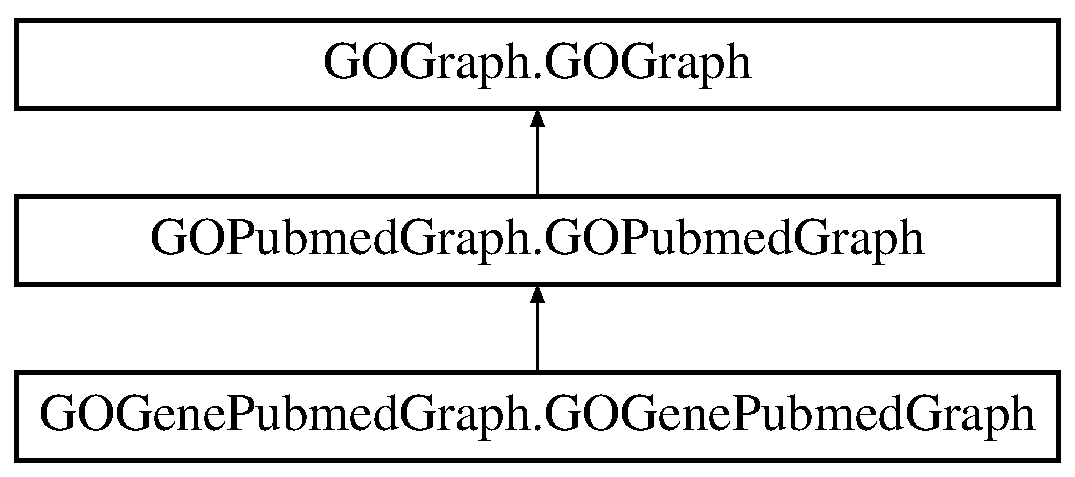
\includegraphics[height=3.000000cm]{class_g_o_pubmed_graph_1_1_g_o_pubmed_graph}
\end{center}
\end{figure}
\subsection*{Public Member Functions}
\begin{DoxyCompactItemize}
\item 
def \hyperlink{class_g_o_pubmed_graph_1_1_g_o_pubmed_graph_a67014838ca4e64ab6302e109cfb38baa}{\_\-\_\-init\_\-\_\-}
\begin{DoxyCompactList}\small\item\em Create a pubmed graph from a \hyperlink{namespace_g_o_graph}{GOGraph}. \item\end{DoxyCompactList}\item 
def \hyperlink{class_g_o_pubmed_graph_1_1_g_o_pubmed_graph_a1cd7af1343cfc3228db50e62ad1d79be}{weight}
\begin{DoxyCompactList}\small\item\em Applies a weight to the graph. \item\end{DoxyCompactList}\item 
def \hyperlink{class_g_o_pubmed_graph_1_1_g_o_pubmed_graph_a9c455a5443e6be4986d7bfbc1ef874c2}{toGOGenePubmedGraph}
\begin{DoxyCompactList}\small\item\em Returns a \hyperlink{namespace_g_o_gene_pubmed_graph}{GOGenePubmedGraph} version of itself. \item\end{DoxyCompactList}\item 
def \hyperlink{class_g_o_pubmed_graph_1_1_g_o_pubmed_graph_a24635a63eda34340ec00919adc165c7c}{getPubMedByNode}
\begin{DoxyCompactList}\small\item\em Returns the associated PubMed IDs for a given node. \item\end{DoxyCompactList}\item 
def \hyperlink{class_g_o_pubmed_graph_1_1_g_o_pubmed_graph_adc36d3c96e860a9db0dee1e60f0f9345}{getNodesByPubMed}
\begin{DoxyCompactList}\small\item\em Returns the associated nodes for a given PubMed ID. \item\end{DoxyCompactList}\end{DoxyCompactItemize}


\subsection{Constructor \& Destructor Documentation}
\hypertarget{class_g_o_pubmed_graph_1_1_g_o_pubmed_graph_a67014838ca4e64ab6302e109cfb38baa}{
\index{GOPubmedGraph::GOPubmedGraph@{GOPubmedGraph::GOPubmedGraph}!\_\-\_\-init\_\-\_\-@{\_\-\_\-init\_\-\_\-}}
\index{\_\-\_\-init\_\-\_\-@{\_\-\_\-init\_\-\_\-}!GOPubmedGraph::GOPubmedGraph@{GOPubmedGraph::GOPubmedGraph}}
\subsubsection[{\_\-\_\-init\_\-\_\-}]{\setlength{\rightskip}{0pt plus 5cm}def GOPubmedGraph.GOPubmedGraph.\_\-\_\-init\_\-\_\- (
\begin{DoxyParamCaption}
\item[{}]{self, }
\item[{}]{gograph, }
\item[{}]{XMLFileName}
\end{DoxyParamCaption}
)}}
\label{class_g_o_pubmed_graph_1_1_g_o_pubmed_graph_a67014838ca4e64ab6302e109cfb38baa}


Create a pubmed graph from a \hyperlink{namespace_g_o_graph}{GOGraph}. 


\begin{DoxyParams}{Parameters}
{\em gograph} & A \hyperlink{namespace_g_o_graph}{GOGraph} to base this graph off of \\
\hline
{\em XMLFileName} & The file containing GO definitions and Pubmed ID information in the format of the OBO in XML \\
\hline
\end{DoxyParams}


Reimplemented from \hyperlink{class_g_o_graph_1_1_g_o_graph_afc10d41165dd1ae6c4cce09102542122}{GOGraph.GOGraph}.



Reimplemented in \hyperlink{class_g_o_gene_pubmed_graph_1_1_g_o_gene_pubmed_graph_a903ad3047a2d1b88fffbdeee60b2045e}{GOGenePubmedGraph.GOGenePubmedGraph}.



\subsection{Member Function Documentation}
\hypertarget{class_g_o_pubmed_graph_1_1_g_o_pubmed_graph_adc36d3c96e860a9db0dee1e60f0f9345}{
\index{GOPubmedGraph::GOPubmedGraph@{GOPubmedGraph::GOPubmedGraph}!getNodesByPubMed@{getNodesByPubMed}}
\index{getNodesByPubMed@{getNodesByPubMed}!GOPubmedGraph::GOPubmedGraph@{GOPubmedGraph::GOPubmedGraph}}
\subsubsection[{getNodesByPubMed}]{\setlength{\rightskip}{0pt plus 5cm}def GOPubmedGraph.GOPubmedGraph.getNodesByPubMed (
\begin{DoxyParamCaption}
\item[{}]{self, }
\item[{}]{pubmed}
\end{DoxyParamCaption}
)}}
\label{class_g_o_pubmed_graph_1_1_g_o_pubmed_graph_adc36d3c96e860a9db0dee1e60f0f9345}


Returns the associated nodes for a given PubMed ID. 


\begin{DoxyParams}{Parameters}
{\em pubmed} & The PubMed ID for which to retrieve the associated nodes: \\
\hline
\end{DoxyParams}
\hypertarget{class_g_o_pubmed_graph_1_1_g_o_pubmed_graph_a24635a63eda34340ec00919adc165c7c}{
\index{GOPubmedGraph::GOPubmedGraph@{GOPubmedGraph::GOPubmedGraph}!getPubMedByNode@{getPubMedByNode}}
\index{getPubMedByNode@{getPubMedByNode}!GOPubmedGraph::GOPubmedGraph@{GOPubmedGraph::GOPubmedGraph}}
\subsubsection[{getPubMedByNode}]{\setlength{\rightskip}{0pt plus 5cm}def GOPubmedGraph.GOPubmedGraph.getPubMedByNode (
\begin{DoxyParamCaption}
\item[{}]{self, }
\item[{}]{goid}
\end{DoxyParamCaption}
)}}
\label{class_g_o_pubmed_graph_1_1_g_o_pubmed_graph_a24635a63eda34340ec00919adc165c7c}


Returns the associated PubMed IDs for a given node. 


\begin{DoxyParams}{Parameters}
{\em goid} & The GOID of the node to retrieve the associated PubMed IDs from \\
\hline
\end{DoxyParams}
\hypertarget{class_g_o_pubmed_graph_1_1_g_o_pubmed_graph_a9c455a5443e6be4986d7bfbc1ef874c2}{
\index{GOPubmedGraph::GOPubmedGraph@{GOPubmedGraph::GOPubmedGraph}!toGOGenePubmedGraph@{toGOGenePubmedGraph}}
\index{toGOGenePubmedGraph@{toGOGenePubmedGraph}!GOPubmedGraph::GOPubmedGraph@{GOPubmedGraph::GOPubmedGraph}}
\subsubsection[{toGOGenePubmedGraph}]{\setlength{\rightskip}{0pt plus 5cm}def GOPubmedGraph.GOPubmedGraph.toGOGenePubmedGraph (
\begin{DoxyParamCaption}
\item[{}]{self}
\end{DoxyParamCaption}
)}}
\label{class_g_o_pubmed_graph_1_1_g_o_pubmed_graph_a9c455a5443e6be4986d7bfbc1ef874c2}


Returns a \hyperlink{namespace_g_o_gene_pubmed_graph}{GOGenePubmedGraph} version of itself. 


\begin{DoxyParams}{Parameters}
{\em gogenegraph} & The \hyperlink{namespace_g_o_gene_graph}{GOGeneGraph} that this graph is to be merged with \\
\hline
\end{DoxyParams}
\hypertarget{class_g_o_pubmed_graph_1_1_g_o_pubmed_graph_a1cd7af1343cfc3228db50e62ad1d79be}{
\index{GOPubmedGraph::GOPubmedGraph@{GOPubmedGraph::GOPubmedGraph}!weight@{weight}}
\index{weight@{weight}!GOPubmedGraph::GOPubmedGraph@{GOPubmedGraph::GOPubmedGraph}}
\subsubsection[{weight}]{\setlength{\rightskip}{0pt plus 5cm}def GOPubmedGraph.GOPubmedGraph.weight (
\begin{DoxyParamCaption}
\item[{}]{self}
\end{DoxyParamCaption}
)}}
\label{class_g_o_pubmed_graph_1_1_g_o_pubmed_graph_a1cd7af1343cfc3228db50e62ad1d79be}


Applies a weight to the graph. 



The documentation for this class was generated from the following file:\begin{DoxyCompactItemize}
\item 
/Users/vickychen/Documents/Projects/myGOGrapher/gographer/\hyperlink{_g_o_pubmed_graph_8py}{GOPubmedGraph.py}\end{DoxyCompactItemize}

\chapter{File Documentation}
\hypertarget{_g_o_gene_graph_8py}{
\section{/Users/vickychen/Documents/Projects/myGOGrapher/gographer/GOGeneGraph.py File Reference}
\label{_g_o_gene_graph_8py}\index{/Users/vickychen/Documents/Projects/myGOGrapher/gographer/GOGeneGraph.py@{/Users/vickychen/Documents/Projects/myGOGrapher/gographer/GOGeneGraph.py}}
}
\subsection*{Classes}
\begin{DoxyCompactItemize}
\item 
class \hyperlink{classgographer_1_1_g_o_gene_graph_1_1_g_o_gene_graph}{gographer.GOGeneGraph.GOGeneGraph}
\end{DoxyCompactItemize}
\subsection*{Packages}
\begin{DoxyCompactItemize}
\item 
package \hyperlink{namespacegographer_1_1_g_o_gene_graph}{gographer.GOGeneGraph}
\item 
package \hyperlink{namespace_g_o_gene_graph}{GOGeneGraph}
\end{DoxyCompactItemize}

\hypertarget{_g_o_gene_pubmed_graph_8py}{
\section{/Users/vickychen/Documents/Projects/myGOGrapher/gographer/GOGenePubmedGraph.py File Reference}
\label{_g_o_gene_pubmed_graph_8py}\index{/Users/vickychen/Documents/Projects/myGOGrapher/gographer/GOGenePubmedGraph.py@{/Users/vickychen/Documents/Projects/myGOGrapher/gographer/GOGenePubmedGraph.py}}
}
\subsection*{Classes}
\begin{DoxyCompactItemize}
\item 
class \hyperlink{class_g_o_gene_pubmed_graph_1_1_g_o_gene_pubmed_graph}{GOGenePubmedGraph.GOGenePubmedGraph}
\end{DoxyCompactItemize}
\subsection*{Packages}
\begin{DoxyCompactItemize}
\item 
package \hyperlink{namespace_g_o_gene_pubmed_graph}{GOGenePubmedGraph}
\end{DoxyCompactItemize}

\hypertarget{_g_o_graph_8py}{
\section{/Users/vickychen/Documents/Projects/myGOGrapher/gographer/GOGraph.py File Reference}
\label{_g_o_graph_8py}\index{/Users/vickychen/Documents/Projects/myGOGrapher/gographer/GOGraph.py@{/Users/vickychen/Documents/Projects/myGOGrapher/gographer/GOGraph.py}}
}
\subsection*{Classes}
\begin{DoxyCompactItemize}
\item 
class \hyperlink{classgographer_1_1_g_o_graph_1_1_g_o_graph}{gographer.GOGraph.GOGraph}
\end{DoxyCompactItemize}
\subsection*{Packages}
\begin{DoxyCompactItemize}
\item 
package \hyperlink{namespacegographer_1_1_g_o_graph}{gographer.GOGraph}
\end{DoxyCompactItemize}

\hypertarget{_g_o_node_8py}{
\section{/Users/vickychen/Documents/Projects/myGOGrapher/gographer/GONode.py File Reference}
\label{_g_o_node_8py}\index{/Users/vickychen/Documents/Projects/myGOGrapher/gographer/GONode.py@{/Users/vickychen/Documents/Projects/myGOGrapher/gographer/GONode.py}}
}
\subsection*{Classes}
\begin{DoxyCompactItemize}
\item 
class \hyperlink{class_g_o_node_1_1_g_o_node}{GONode.GONode}
\end{DoxyCompactItemize}
\subsection*{Packages}
\begin{DoxyCompactItemize}
\item 
package \hyperlink{namespace_g_o_node}{GONode}
\end{DoxyCompactItemize}

\hypertarget{_g_o_obo_xml_handler_8py}{
\section{/Users/vickychen/Documents/Projects/myGOGrapher/gographer/GOOboXmlHandler.py File Reference}
\label{_g_o_obo_xml_handler_8py}\index{/Users/vickychen/Documents/Projects/myGOGrapher/gographer/GOOboXmlHandler.py@{/Users/vickychen/Documents/Projects/myGOGrapher/gographer/GOOboXmlHandler.py}}
}
\subsection*{Classes}
\begin{DoxyCompactItemize}
\item 
class \hyperlink{classgographer_1_1_g_o_obo_xml_handler_1_1_g_o_obo_xml_handler}{gographer.GOOboXmlHandler.GOOboXmlHandler}
\end{DoxyCompactItemize}
\subsection*{Packages}
\begin{DoxyCompactItemize}
\item 
package \hyperlink{namespacegographer_1_1_g_o_obo_xml_handler}{gographer.GOOboXmlHandler}
\end{DoxyCompactItemize}

\hypertarget{_g_o_pubmed_graph_8py}{
\section{/Users/vickychen/Documents/Projects/myGOGrapher/gographer/GOPubmedGraph.py File Reference}
\label{_g_o_pubmed_graph_8py}\index{/Users/vickychen/Documents/Projects/myGOGrapher/gographer/GOPubmedGraph.py@{/Users/vickychen/Documents/Projects/myGOGrapher/gographer/GOPubmedGraph.py}}
}
\subsection*{Classes}
\begin{DoxyCompactItemize}
\item 
class \hyperlink{class_g_o_pubmed_graph_1_1_g_o_pubmed_graph}{GOPubmedGraph.GOPubmedGraph}
\end{DoxyCompactItemize}
\subsection*{Packages}
\begin{DoxyCompactItemize}
\item 
package \hyperlink{namespace_g_o_pubmed_graph}{GOPubmedGraph}
\end{DoxyCompactItemize}

\hypertarget{test_8py}{
\section{/Users/vickychen/Documents/Projects/myGOGrapher/gographer/test.py File Reference}
\label{test_8py}\index{/Users/vickychen/Documents/Projects/myGOGrapher/gographer/test.py@{/Users/vickychen/Documents/Projects/myGOGrapher/gographer/test.py}}
}
\subsection*{Packages}
\begin{DoxyCompactItemize}
\item 
package \hyperlink{namespacetest}{test}
\end{DoxyCompactItemize}
\subsection*{Variables}
\begin{DoxyCompactItemize}
\item 
string \hyperlink{namespacetest_a4ee7d63d9426ae32ba96ad2f0e171511}{test.location} = \char`\"{}./go\_\-daily-\/termdb.obo-\/xml\char`\"{}
\item 
tuple \hyperlink{namespacetest_a49256f3800de70e9aabf11ea0c3bb8e1}{test.GOGraphtest} = GOGraph(\char`\"{}biological\_\-process\char`\"{}, location)
\item 
string \hyperlink{namespacetest_afe7b4432163ad853f4fcd650d0ecab8c}{test.descrip} = 'The chemical reactions and pathways involving (R)-\/4-\/hydroxymandelate, the anion of a hydroxylated derivative of mandelate (alpha-\/hydroxybenzeneacetate).'
\item 
string \hyperlink{namespacetest_a1429061289985226ca44c2e4e888d77e}{test.namespace} = 'biological\_\-process'
\item 
string \hyperlink{namespacetest_adb8b1e2a5df72522e42bc012571e75cd}{test.assoc} = \char`\"{}./gene\_\-association.goa\_\-human\char`\"{}
\item 
tuple \hyperlink{namespacetest_ab48a47ac8dcf21d32cff24c492f085c1}{test.GOGenetest} = GOGeneGraph(GOGraphtest,assoc)
\item 
tuple \hyperlink{namespacetest_a836657c6fd789469b5cbdd3c88513f7f}{test.genes} = set(\mbox{[}('P05091', ''), ('Q8NE62', ''), ('P47895', ''), ('P48448', ''), ('P00326', ''), ('P43353', ''), ('P08319', ''), ('P07327', '')\mbox{]})
\item 
tuple \hyperlink{namespacetest_a6b190968f9c7fc0593c63df10224e21a}{test.propGenes} = set(\mbox{[}('Q8NE62', ''), ('P47895', ''), ('O43704', ''), ('P48448', ''), ('P43353', ''), ('P05091', ''), ('P00326', ''), ('P08319', ''), ('P07327', '')\mbox{]})
\item 
tuple \hyperlink{namespacetest_aa8cc3a0b86b4a37acf878753845ac845}{test.nodesByGene} = set(\mbox{[}'GO:0006066', 'GO:0008152'\mbox{]})
\item 
tuple \hyperlink{namespacetest_a2565076d50762c7d466830ecbabb1671}{test.GOPubmedtest} = GOPubmedGraph(GOGraphtest,assoc)
\item 
tuple \hyperlink{namespacetest_aa3b15c95748b55bb3ace649b708b6133}{test.pubmed} = set(\mbox{[}('2347582', ''), ('7698756', ''), ('1306115', ''), ('3466164', ''), ('7828891', ''), ('8890755', '')\mbox{]})
\item 
tuple \hyperlink{namespacetest_adc1d0604ecf3fb36f0df45313768ab39}{test.propPubmed} = set(\mbox{[}('10203017', ''), ('7959792', ''), ('9473496', ''), ('7663508', ''), ('10692104', ''), ('6548414', ''), ('3466164', ''), ('10359671', ''), ('11300766', ''), ('11254442', ''), ('9000139', ''), ('10022914', ''), ('8822211', ''), ('10373482', ''), ('1695324', ''), ('1374385', ''), ('3800996', ''), ('12882974', ''), ('3755672', ''), ('9500206', ''), ('8890755', ''), ('8353497', ''), ('9733774', ''), ('9263035', ''), ('8707889', ''), ('9295054', ''), ('7698756', ''), ('8333863', ''), ('7912130', ''), ('9207799', ''), ('11597136', ''), ('9305759', ''), ('2347582', ''), ('10101297', ''), ('8359595', ''), ('11606197', ''), ('1918003', ''), ('1306115', ''), ('9268630', ''), ('9299468', ''), ('10382971', ''), ('9463486', ''), ('11179693', ''), ('9237672', ''), ('7828891', ''), ('9207021', ''), ('2110361', '')\mbox{]})
\end{DoxyCompactItemize}

\printindex
\end{document}
